
\begin{itemize}
	\item Коэффициент аннигилляции $aT_{\odot}^2 = A(t = T_{\odot})/C^2$ находится из рещшения линейного уравнения.
\end{itemize}
\begin{figure}[!h]
	\centering
	\only<1>{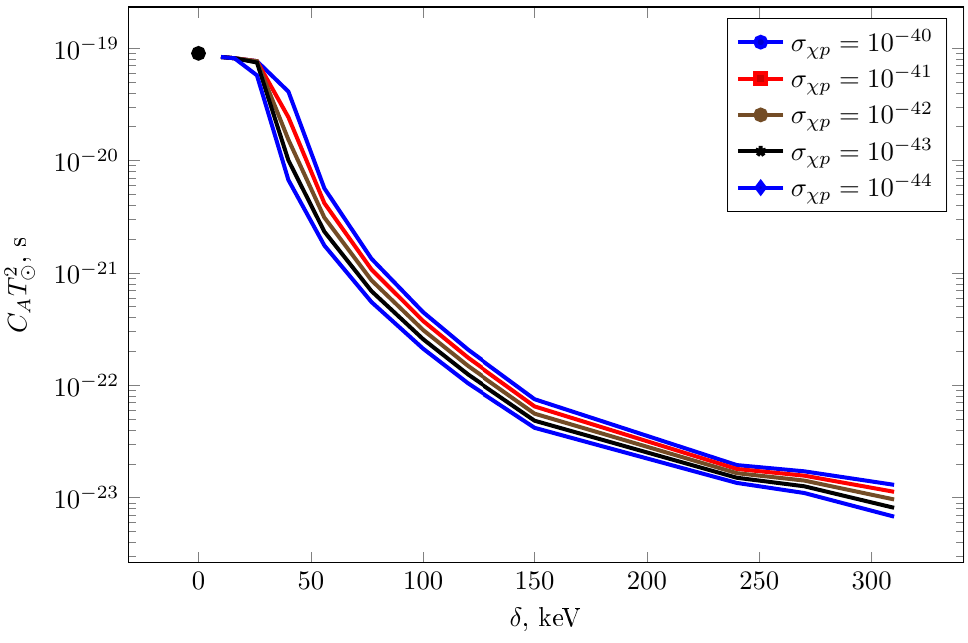
\includegraphics[width=0.7\textwidth]{images/AnnCoeff.png}
	\caption{Коэффициент аннигиляции для нераспадающейся ТМ $m_{\chi} = 100 \text{GeV}$}
	}
	\only<2>{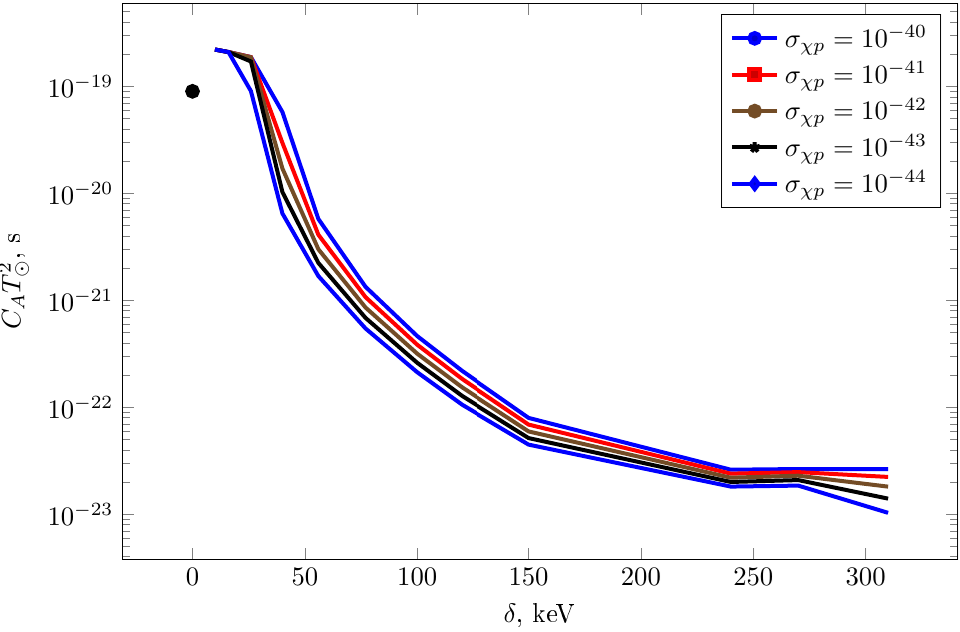
\includegraphics[width=0.7\textwidth]{images/AnnCoeffFD.png}
	\caption{Коэффициент аннигиляции для распадающейся ТМ $m_{\chi} = 100 \text{GeV}$}
	}
\end{figure}